\documentclass[../main.tex]{subfiles}

\begin{document}
\chapter{Taylorreihen und Potenzreihen}
\section{Taylorentwicklung}
Sei $f \colon \mathbb{R} \to \mathbb{R}$ differenzierbar.
Dann hat $f$ in  jedem Punkt $p \in \mathbb{R}$ eine Dreigliedentwicklung
der Form
\[
  f(p+ h) = f(p) + {(Df)}_p(h) + {(Rf)}_p(h).
\]
Insbesondere gilt für $p = 0$ und $h = x$, dass
\begin{align*}
  f(x) &= f(0) + {(Df)}_0(x) + {(Rf)}_0(x) \\
       &= f(0) + f'(0) \cdot x + {(Rf)}_0(x).
\end{align*}

\begin{definition}
  Eine Funktion $f \colon \mathbb{R} \to \mathbb{R}$ heisst $n$-\emph{mal
  differenzierbar}, falls alle Ableitungen $f', f'', \dots, f^{(n)}$ existieren.
  Weiter heisst eine Funktion $f$ 
  $n$-\emph{mal stetig differenzierbar} falls $f$ 
  eine $n$-mal differenzierbare Funktion und 
  $f^{(n)} \colon \mathbb{R} \to \mathbb{R}$ stetig ist.
\end{definition}


Sei nun $f \colon \mathbb{R} \to \mathbb{R}$ zweimal differenzierbar.
Das heisst, die Funktion $f' \colon \mathbb{R} \to \mathbb{R}$ ist differenzierbar.
Dann erhalten wir
\[
  f'(x) = f'(0) + f''(0) \cdot x + {(Rf')}_0 (x).
\]
Wir erhalten aus
\[
  f(x) - f(0)
   = \int_{0}^{x} f'(t) \, dt,
\]
dass
\begin{align*}
  f(x) 
  & = f(0) + \int_{0}^{x} f'(0) + f''(0) \cdot t + {(Rf')}_0(t) \, dt  \\
  & = f(0) + f'(0) \cdot x + f''(0) \cdot \frac{x^2}{2} + \int_{0}^{x} {(Rf')}_0(t) \, dt.
\end{align*}
Durch Iteration dieses Verfahrens erhalten wir folgenden Satz.

\newpage
\begin{theorem}[Brook Taylor, ca. 1715]\label{thm:taylor}
  Sei $f \colon \mathbb{R} \to \mathbb{R}$ eine
  $n$-mal stetig differenzierbare Funktion für $n \in \mathbb{N}$ mit $n \geq 1$.
  Dann besitzt $f$ eine Entwicklung
  mit $n + 2 $ Gliedern der Form
  \[
    f(x) = \sum_{k=0}^{n} \frac{f^{(k)}(0)}{k!}x^k + {(Rf)}_n(x),
  \]
  wobei der Restterm ${(Rf)}_n(x)$ relativ klein in
  $|x|^n$ ist. Das heisst, für alle $ \varepsilon > 0$
  existiert $\delta > 0$ so, dass für alle $x \in \mathbb{R}$ mit
  $|x| \leq \delta$ gilt, dass
  \[
    |{(Rf)}_n(x)| \leq \varepsilon \cdot |x|^n.
  \]
\end{theorem}

\begin{proof}
  Wir beweisen diesen Satz durch Induktion über $n \in \mathbb{N}$.
  Die Verankerung bei $n = 1$ ist bloss die Definition der Differenzierbarkeit
  via die Dreigliedentwicklung.
  Wir treffen die Induktionsannahme, dass die Aussage für $n-1$ gilt.
  Sei $f \colon \mathbb{R} \to \mathbb{R}$ eine $n$-mal stetig differenzierbare Funktion.
  Das heisst, $f'$ ist eine $(n-1)$-mal stetig differenzierbare Funktion.
  Nach der Induktionsannahme hat $f'$ eine Entwicklung der Form
  \[
    f'(x) = \sum_{k=0}^{n-1} \frac{f^{(k+1)}(0)}{k!}x^k + {(Rf')}_{n-1}(x).
  \]
  Der Hauptsatz der Differential- und Integralrechnung liefert
  \begin{align*}
    f(x) - f(0) & = \int_{0}^{x} f'(t) \, dt \\
                & = \int_{0}^{x} \sum_{k=0}^{n-1} \frac{f^{k+1}(0)}{k!}t^k
                + {(Rf')}_{n-1}(t)\, dt.
  \end{align*}
  Daraus folgt, dass
  \[
    f(x) = f(0) + \sum_{k=0}^{n-1} \frac{f^{(k+1)}(0)}{k!} \int_{0}^{x} t^k \, dt
    + \int_{0}^{x} {(Rf')}_{n-1}(t) \, dt.
  \]
  Setzen wir
  \[
    {(Rf)}_n(x) = \int_{0}^{x} {(Rf')}_{n-1}(t) \, dt,
  \]
  so erhalten wir
  \begin{align*}
    f(x) & = f(0) + \sum_{k=0}^{n-1} \frac{f^{(k+1)}(0)}{(k+1)!}x^{k+1} + {(Rf)}_n(x) \\
         & = \sum_{\ell=0}^{n} \frac{f^{(\ell)}(0)}{\ell!}x^{\ell} + {(Rf)}_n(x).
  \end{align*}
  Wir behaupten nun, dass ${(Rf)}_n(x)$ relativ klein in $|x|^n$ ist.
  Sei dazu $\varepsilon > 0$ vorgegeben. Dann existiert $\delta > 0$,
  so dass für alle $t \in \mathbb{R}$ mit $|t| \leq \delta$ gilt,
  dass
  \[
    |{(Rf')}_{n-1}(t)| \leq \varepsilon \cdot |t|^{n-1}.
  \]
  Schätze für $0 \leq x \leq \delta$ ab, dass
  \begin{align*}
    |{(Rf)}_n(x)| 
    &= \left| \int_{0}^{x} {(Rf')}_{n-1}(t) \, dt \right|  \\
    &\leq \int_{0}^{x} |{(Rf')}_{n-1}(t)| \, dt \\
    &\leq \int_{0}^{x} \varepsilon \cdot |t|^{n-1} \, dt \\
    &= \int_{0}^{x} \varepsilon \cdot t^{n-1} \, dt \\
    &= \varepsilon \cdot \frac{x^n}{n} \\
    &\leq \varepsilon \cdot |x|^n.
  \end{align*}
  Der Fall $-\delta \leq x \leq 0$ ist ähnlich.
  Die Ungleichung
  \[
    \left| \int_{0}^{x} g(t) \, dt \right| \leq \int_{0}^{x} |g(t)| \, dt
  \]
  gilt für alle Riemann-integrierbaren $g \colon [0, x] \to \mathbb{R}$
  und $x \geq 0$.
  Schätze dazu alle Ober- und Untersummen ab.
  Abbildung~\ref{fig:riemann-integral} liefert auch hier eine geometrische Erklärung.
  Eine ähnliche Abschätzung gilt für $x < 0$, da nach Konvention
  \[
    \int_{0}^{x} g(t) \, dt = - \int_{x}^{0} g(t) \, dt
  \]
  gilt.
  Die Funktion $t \mapsto {(Rf')}_{n-1}(t)$ ist Riemann-integrierbar, da
  \[
    {(Rf')}_{n-1}(t) = f'(t) - \sum_{k=0}^{n-1} \frac{f^{k+1}(0)}{k!}t^k
  \]
  die Summe einer stetigen Funktion mit einem Polynom ist.
\end{proof}

\begin{zusatz}
  Es existiert ein $\zeta \in [0, x]$ mit 
  \[
    {(Rf)}_n(x) = \frac{f^{(n)}(\zeta)}{(n+1)!}x^{n+1},
  \]
  genannt Restglied von Lagrange.
\end{zusatz}

Der Beweis ist in Abschnitt 61 in~\cite{heuser} zu finden.
Der Spezialfall $n = 0$ ist bloss eine Umformulierung des Mittelwertsatzes,
da dort
\[
  f(x) = f(0) + f'(\zeta) \cdot x
\]
steht.

\begin{definition}
  Sei $f \colon \mathbb{R} \to \mathbb{R}$ unendlich oft differenzierbar,
  das heisst, für alle $k \in \mathbb{N}$ existiert die $k$-te Ableitung
  $f^{(k)} \colon \mathbb{R} \to \mathbb{R}$.
  Die \emph{Taylorreihe} oder \emph{Taylorentwicklung} von $f$ bei $0$ ist die formale Reihe
  \[
    Tf(x) = \sum_{k=0}^{\infty} \frac{f^{(k)}(0)}{k!}x^k.
  \]
\end{definition}

\begin{questions}
  Sei $f \colon \mathbb{R} \to \mathbb{R}$ unendlich oft
  differenzierbar.
  \begin{enumerate}[(1)]
    \item Ist die Reihe $Tf(x)$ für alle $x \in \mathbb{R}$ konvergent?
    \item Nehme an, dass $Tf(x)$ konvergiert. Gilt dann $f(x) = Tf(x)$?
  \end{enumerate}
\end{questions}

Leider ist die Antwort auf beide Fragen im Allgemeinen nein.

\begin{definition}
  Eine unendlich oft differenzierbare Funktion
  $f \colon \mathbb{R} \to \mathbb{R}$ heisst \emph{analytisch},
  falls für alle $x \in \mathbb{R}$ die Reihe
  $Tf(x)$ konvergiert und $Tf(x) = f(x)$ gilt.
\end{definition}

\begin{examples}
  \leavevmode
  \begin{enumerate}[(1)]
    \item Seien $a_0, \dots, a_n \in \mathbb{R}$ und
      $f \in \mathbb{R}[x]$ mit
      \[
        f(x) = a_0 + a_1 x + a_2 x^2 + \cdots +a_n x^{n}.
      \]
      Berechne, dass
      \begin{itemize}
        \item $f(0) = a_0$,
        \item $f'(0)$ = $a_1$,
        \item $f''(0) = 2a_2$,
        \item \dots,
        \item $f^{(k)}(0) = k! \cdot a_k$ für $k \leq n$,
        \item $f^{(k)}(0) = 0$ für $k > n$.
      \end{itemize}
      Es folgt, dass
      \[
        Tf(x) = \sum_{k=0}^{\infty} \frac{f^{(k)}(0)}{k!}x^k
        = \sum_{k=0}^{\infty} \frac{k! \cdot a_k}{k!}x^k = f(x).
      \]
      Also sind Polynome analytisch.
    \item Betrachte die Funktion
      \begin{align*}
        \exp \colon \mathbb{R} & \to \mathbb{R} \\
        x & \mapsto e^x.
      \end{align*}
      Dann gilt $\exp'(x) = e^x$. Also ist $\exp$ unendlich oft differenzierbar
      und für alle $k \in \mathbb{N}$ gilt $\exp^{(k)}(0) = e^0 = 1$.
      Somit ist
      \[
        T\exp(x) = \sum_{k=0}^{\infty} \frac{f^{(k)}(0)}{k!}x^k
        = \sum_{k=0}^{\infty} \frac{x^k}{k!} = e^x.
      \]
      Also ist $T\exp(x)$ konvergent, wie wir bereits in früheren Betrachtungen
      gesehen haben, und $T\exp(x) = e^x$ für alle $x \in \mathbb{R}$.
      Somit ist die Exponentialfunktion analytisch.
    \item Betrachte die Funktion
      \begin{align*}
        f \colon \mathbb{R} & \to \mathbb{R} \\
        x & \mapsto 
        \begin{cases}
          0 & x = 0,\\
          e^{-1/x^2} & x \neq 0.
        \end{cases}
      \end{align*}
      Wir werden sehen, dass $Tf = 0$ die Nullfunktion ist.
      Dazu schätzen wir zuerst für alle $x \neq 0$ die Ableitungen
      $f^{(k)}(x)$ wie folgt ab. Berechne
      \begin{itemize}
        \item $f'(x) = 2/x^3 \cdot e^{-1/x^2}$,
        \item $f''(x) = {(2/x^3)}^2 \cdot e^{-1/x^2} - 6/x^4 \cdot e^{- 1/x^2}$.
      \end{itemize}
      Wir behaupten, dass für alle $k \geq 1$ ein Polynom $p_k \in \mathbb{R}[x]$ 
      vom Grad höchstens $3k$ existiert,
      so dass
      \[
        f^{(k)}(x) = \frac{p_k(x)}{x^{3k}} \cdot e^{-1/x^2}.
      \]
      Der Beweis ist ein kurzer Induktionsbeweis. Die Verankerung bei $k = 1$ 
      haben wir bereits oben gezeigt. Für den Induktionsschritt von $k$ zu
      $k + 1$ berechnen wir
      \begin{align*}
         \left( \frac{p_k(x)}{x^{3k}} e^{-1/x^2}\right)'
         &= \left( \frac{p_k'(x)}{x^{3k}} - \frac{3k \cdot p_k(x)}{x^{3k+1}} \right)
         \cdot e^{-1/x^2}
         + \frac{p_k(x)}{x^{3k} \cdot 2/x^3} \cdot e^{-1/x^2}\\
         &= \frac{p_{k+1}(x)}{x^{3k+3}} \cdot e^{-1/x^2},
      \end{align*}
      wobei der Grad von $p_{k+1}$ höchstens $3(k+1)$ ist.

      Als nächstes zeigen wir, dass für alle $k \in \mathbb{N}$ die Ableitung
      $f^{(k)}(0)$ existiert und $f^{(k)}(x) = 0$ ist.
      Berechne
      \begin{align*}
        f'(0)
        & = \lim_{x \to 0} \frac{f(x) - f(0)}{x}\\
        & = \lim_{x \to 0} \frac{e^{-1/x^2}}{x}\\
        & = \lim_{x \to 0} \frac{1}{x \cdot e^{1/x^2}} \\
        & = \lim_{z \to \infty} \frac{z}{e^{z^2}} \\
        & = 0,
      \end{align*}
      womit wir bei $k = 1$ verankert haben.
      Für den Induktionsschritt von $k$ zu $k + 1$ berechne
      \begin{align*}
        f^{(k+1)}(0)
        & = \lim_{x \to 0} \frac{f^{(k)}(x) - f^{(k)}(0)}{x}\\
        & = \lim_{x \to 0} \frac{f^{(k)}(x)}{x}\\
        & = \lim_{x \to 0} \frac{p_k(x)}{x^{3k+1}} \cdot e^{-1/x^2}\\
        & = \lim_{z \to \infty} \frac{p_k(1/z) \cdot z^{3k+1}}{e^{z^2}} \\
        & = 0.
      \end{align*}
      Also konvergiert die Taylorreihe $Tf$ für alle $x \in \mathbb{R}$,
      aber nur für $x = 0$ gilt $Tf(x) = f(x)$.
      Also ist $f$ nicht analytisch.
      Das beantwortet Frage (2) negativ.

      \begin{figure}[htb]
        \centering
        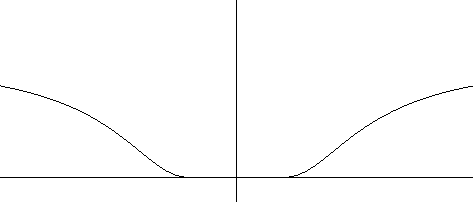
\includegraphics{images/non-analytic}
        \caption{Die Funktion $x \mapsto e^{-1/x^2}$}%
        \label{fig:non-analytic}
      \end{figure}

    \item Betrachte die Funktion
      \begin{align*}
        f \colon \mathbb{R} \setminus \{1\} & \to \mathbb{R} \\
        x & \mapsto \frac{1}{1-x}.
      \end{align*}
      Dann ist $f$ unendlich oft differenzierbar auf
      $\mathbb{R} \setminus \{1\}$. Berechne
      \begin{align*}
        f'(x) & = -\frac{1}{{(1 - x)}^2} \cdot (-1)
        = {(1 - x)}^{-2},\\
        f''(x) &= -2 \cdot \frac{1}{{(1-x)}^3} = {(1 - x)}^{-3},
      \end{align*}
      und allgemein
      \[
        f^{(k)}(x) = k! \cdot {(1 - x)}^{-(k + 1)}.
      \]
      Insbesondere ist $f^{(k)}(0) = k!$. 
      Die Taylorreihe ist also
      \[
        Tf(x) = \sum_{k=0}^{\infty} \frac{k!}{k!} x^k
        = \sum_{k=0}^{\infty} x^k.
      \]
      Das ist eine geometrische Reihe, die genau konvergent für
      $|x| < 1$ ist.
      Das ist aber noch nicht ein Gegenbeispiel zur Frage (1),
      da $f$ nicht auf ganz $\mathbb{R}$ unendlich oft
      differenzierbar ist.
      Wir bemerken aber, dass für $|x| < 1$ gilt, dass
      \[
        \sum_{k=0}^{\infty} x^k = \frac{1}{1-x}.
      \]
      Also stimmt $Tf(x)$ dort, wo die Reihe konvergent ist,
      mit $f$ überein.

    \item Definiere zuerst eine Hilfsfunktion
      \begin{align*}
        h \colon \mathbb{R} & \to \mathbb{R} \\
        x & \mapsto 
        \begin{cases}
          0, & x \leq 0,\\
          e^{-1/x^2}, & x > 0.
        \end{cases}
      \end{align*}
      Dann ist $h$ unendlich oft auf ganz $\mathbb{R}$ 
      differenzierbar, und für alle $k \in \mathbb{N}$ 
      gilt 
      \[
      h^{(k)}(0) = 0,
      \]
      analog zum Beispiel (3).
      Definiere nun
      \begin{align*}
        \overline h \colon \mathbb{R} & \to \mathbb{R} \\
        x & \mapsto h(x - 1/3) \cdot h(2/3 - x).
      \end{align*}
      Auch $\overline h$ ist unendlich oft differenzierbar.
      Es gilt:
      \begin{itemize}
        \item Für $x \leq 1/3$ ist $\overline h(x) = 0$,
        \item Für $x \geq 2/3$ ist $\overline h(x) = 0$,
        \item Für $x \in (1/3, 2/3)$ ist $\overline h(x) > 0$.
      \end{itemize}
      Definiere
      \begin{align*}
        H \colon \mathbb{R} & \to \mathbb{R} \\
        x & \mapsto 
        c \cdot 
        \int_{0}^{x} \overline h(t) \, dt.
      \end{align*}
      
      \begin{figure}[htb] 
        \centering
        \begin{minipage}{0.50\textwidth}
          \centering
          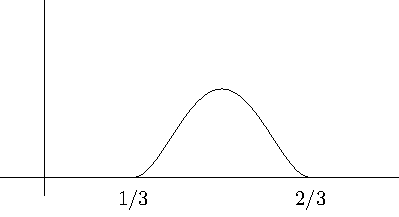
\includegraphics{images/partition-integrand}
        \end{minipage}%
        \begin{minipage}{0.50\textwidth}
          \centering
          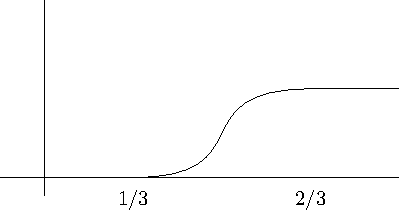
\includegraphics{images/partition-integrated}
        \end{minipage}%
        \caption{Konstruktion von $H$}%
        \label{fig:partition}
      \end{figure}

      Die Funktion $H$ ist unendlich oft differenzierbar,
      da $H'(x) = \overline c \cdot h(x)$ und es gilt:
       \begin{itemize}
         \item Für $x \leq 1/3$ ist $H(x) = 0$.
         \item Auf $\mathbb{R}_{\geq 2/3}$ ist $H$ konstant.
      \end{itemize}
      Wähle nun $c > 0$ so, dass $H$ 
      auf $\mathbb{R}_{\geq 2/3}$ konstant $1$ ist,
      das heisst
      \[
        c = \left. 1 \middle/ \int_{0}^{1} \overline h(t) \, dt.\right.
      \]
      
      Betrachte nun die Funktion
      \begin{align*}
        f \colon \mathbb{R} & \to \mathbb{R} \\
        x & \mapsto 
        \begin{cases}
          1/(1- x) \cdot (1 - H(x)), & x < 1,\\
          0, x \geq 1.
        \end{cases}
      \end{align*}
      Nun ist $f$ auf $\mathbb{R} \setminus \{1\}$
      unendlich oft differenzierbar und es gilt:
      \begin{itemize}
        \item Für $x \leq 1/3$ ist $H(x) = 0$, also
          ist $f(x) = 1/(1- x)$.
        \item Für $x \geq 2/3$ ist $H(x) = 1$, also
          ist $f(x) = 0$.
      \end{itemize}
      Wir folgern, dass $f$ auch im Punkt $x = 1$ 
      unendlich oft differenzierbar ist,
      da $f$ auf dem offenen Intervall $(2/3, 4/3)$ konstant ist.
      Aus
      \[
        f|_{(-1/3, 1/3)}(x) = \frac{1}{1-x}
      \]
      folgt, dass
      \[
        Tf(x) = \sum_{k=0}^{\infty} x^k.
      \]
      Dies beantwortet die Frage (1): Die Funktion $f \colon \mathbb{R} \to \mathbb{R}$ 
      ist unendlich oft differenzierbar, aber $Tf(x)$ ist nur für $|x| < 1$ konvergent.
      Dieser Prozess heisst \emph{Zerlegung der Eins} und ist in der Differentialtopologie
      ein zentraler Trick.
  \end{enumerate}
\end{examples}

\subsection*{Taylorentwicklung in beliebigen Punkten}
Folgender Satz ist bloss eine Verallgemeinerung von Theorem~\ref{thm:taylor}.

\begin{theorem}
  Sei $f \colon \mathbb{R} \to \mathbb{R}$ $n$-mal stetig differenzierbar
  und $p \in \mathbb{R}$ vorgegeben.
  Dann besitzt $f$ im Punkt $p$ eine Entwicklung der Form
  \[
    Tf(x) = \sum_{k=0}^{n} \frac{f^{(k)}(p)}{k!} {(x - p)}^k + {(Rf)}_n(x - p),
  \]
  wobei ${(Rf)}_n (x - p)$ relativ klein in $|x - p|^n$ ist.
\end{theorem}

\begin{proof}
  Wende Theorem~\ref{thm:taylor} über die Taylorentwicklung im Nullpunkt
  auf die Funktion
  \begin{align*}
    h \colon \mathbb{R} & \to \mathbb{R} \\
    x & \mapsto f(x + p)
  \end{align*}
  an. Wir erhalten
  \[
    h(x) = \sum_{k=0}^{n} \frac{h^{(k)}(0)}{k!} x^k + {(Rh)}_n(x),
  \]
  wobei ${(Rh)}_n(x)$ relativ klein in $|x|^n$ ist.
  Mit $f(x) = h(x - p)$ und $h^{(k)}(0) = f^{(k)}(p)$ erhalten wir
  \[
    f(x) = h(x - p) = \sum_{k=0}^{n} \frac{f^{(k)}(p)}{k!}{(x-p)}^k + {(Rh)}_n(x-p).
    \qedhere
  \]
\end{proof}

\begin{examples}
  \leavevmode
  \begin{enumerate}[(1)]
    \item Sei $f(x) = a_0 + a_1 x + \cdots + a_n x^n$.
      Sei $p \in \mathbb{R}$ beliebig.
      Es gilt $f^{(n)}(p) = n! \cdot a_n$ und
      $f^{(n+1)}(p) = 0$. Also kann man $f(x)$ schreiben als
      \[
        f(x) = \sum_{k=0}^{n} b_k {(x - p)}^k
      \]
      mit $b_n = a_n$. Wir machen keine Aussage über die weiteren $b_k$.
    \item Betrachte die Funktion  $\log \colon \mathbb{R}_{>0} \to \mathbb{R}$.
      Wir berechnen die Taylorentwicklung von $\log$ bei $p = 1$.
      Berechne $\log(1) = 0$. Die Ableitungen des Logarithmus sind
      \[
        \log^{(k)}(x) = {(-1)}^{k+1} \frac{(k-1)!}{x^k},
      \]
      also gilt $f^{(k)}(1) = {(-1)}^{k+1} (k-1)!$.
      Wir folgern, dass
      \[
        T\log(x) = \sum_{k=0}^{\infty} \frac{{(-1)}^{k+1}(k-1)!}{k!}{(x-1)}^k
        = \sum_{k=1}^{\infty} \frac{{(-1)}^{k+1}}{k}{(x-1)}^k.
      \]
      Diese Reihe ist konvergent für alle $x \in (0, 2)$.
      Vergleiche sie dazu mit der geometrischen Reihe.
      Für $x = 0$ erhalten wir $-1 -1/2 - 1/3 - \cdots$, was divergiert.
      Für $x = 2$ erhalten wir $1 - 1/2 + 1/3 - 1/4 + \cdots$, was nach
      dem Leibnizkriterium konvergent ist.

      Wir haben nun also eine Taylorreihe $T\log$ für $\log$ gefunden.
      Für welche $x$ konvergiert nun $T\log(x)$?
      Berechne dazu für $|z| < 1$, dass
      \begin{align*}
         \log(1 + z) - \log(1)
         &= \int_{1}^{1+z} \frac{1}{t} \, dt  \\
         &= \int_{0}^{z} \frac{1}{1+s} \, ds.
      \end{align*}
      Aus $|z| < 1$ folgt auch $|s| < 1$ für $s \in [0, z]$, also folgt
      durch vertauschen des Integrals mit der Summe (was wir später rechtfertigen),
      dass
      \begin{align*}
        \log(1+z)
        & = \int_{0}^{z} \left( \sum_{k=0}^{\infty} {(-1)}^k s^k \right) \, ds\\
        &= \sum_{k=0}^{\infty} {(-1)}^k \int_{0}^{z} s^k \, ds\\
        &= \sum_{k=0}^{\infty} {(-1)}^k \frac{z^{k+1}}{k+1}\\
        &= \sum_{k=1}^{\infty} {(-1)}^{k+1} \frac{z^k}{k},
      \end{align*}
      Im Allgemeinen dürfen wir die Reihenfolge des Summieren und Integrieren
      nicht vertauschen. In dieser Situation dürfen wir das aber, 
      siehe
      Proposition~\ref{prop:swap-limit-integral} unten.
      Dieser Trick funktioniert sogar im Grenzfall $z = 1$. Es gilt also
      \[
        \log(2) = \sum_{\ell = 1}^{\infty} \frac{{(-1)}^{\ell+1}}{\ell}
        = 1 - 1/2 + 1/3 - 1/4 + \dots.
      \]
      Siehe dazu den Grenzwertsatz von Abel, Proposition~\ref{prop:abel-grenzwertsatz} unten.
      Wir folgern, dass $T\log(x) = \log(x)$ für alle $x \in \mathbb{R}$
      mit $0 < x \leq 2$.
  \end{enumerate}
\end{examples}


\section{Konvergenzradius von Potenzreihen}\label{sec:radius}
Seien $a_0, a_1, a_2, \dots \in \mathbb{R}$.
Die formale Reihe
\[
  P(x) = \sum_{k=0}^{\infty} a_k x^k
\]
heisst \emph{Potenzreihe}.

\begin{definition}
  Eine Zahl $r \in \mathbb{R} \cup \{\infty\}$ heisst
  \emph{Konvergenzradius} der Potenzreihe 
  \[
    P(x) = \sum_{k=0}^{\infty} a_k x^k,
  \]
  falls
  \begin{enumerate}[(i)]
    \item für alle $x \in \mathbb{R}$ mit $|x| < r$ ist $P(x)$ konvergent,
    \item für alle $x \in \mathbb{R}$ mit $|x| > r$ ist $P(x)$ divergent.
  \end{enumerate}
\end{definition}

Die Definition des Konvergenzradius macht keine Aussage über den Fall $|x| = r$.
Bemerke, dass es a priori nicht klar ist, dass jede Potenzreihe
einen Konvergenzradius hat. Wir werden aber zeigen, dass das aber trotzdem gilt.

\begin{examples}
  \leavevmode
  \begin{enumerate}[(1)]
    \item Die Potenzreihe
      \[
        P(x) = \sum_{k=0}^{\infty} \frac{x^k}{k!}
      \]
      konvergiert für alle $x \in \mathbb{R}$, 
      Also ist ihr Konvergenzradius $r = \infty$.
    \item Die Potenzreihe
      \[
        P(x) = \sum_{k=0}^{\infty} x^k
      \]
      konvergiert für $|x| < 1$. Für $|x| \geq 1$ ist ${(x^{k})}_{k \in \mathbb{N}}$ keine
      Nullfolge, also ist der Konvergenzradius $r = 1$.
    \item Die Potenzreihe
      \[
        P(x) = \sum_{k=1}^{\infty} \frac{x^k}{k}
      \]
      ist konvergent für genau diejenigen $x \in \mathbb{R}$ mit $-1 \leq x < 1$.
      Also ist auch hier der Konvergenzradius $r = 1$.
      Tatsächlich gilt für $|x| > 1$, dass $P(x)$ divergent ist.
      Das ist klar für $x > 1$. Für $x < -1$ schreibe
      $x = -(1 + \varepsilon)$ mit $\varepsilon > 0$.
      Dann gilt 
      \[
        |x|^k = (1 + \varepsilon)^k \geq 1 + k \varepsilon
      \]
      nach der Bernoulli-Ungleichung. Folglich ist $|x|^k/k \geq \varepsilon$ 
      für alle $k \geq 1$, also ist $x^k/k$ keine Nullfolge.
    \item Die Potenzreihe
      \[
        \sum_{k=1}^{\infty} \frac{1}{k^2}x^k
      \]
      konvergiert genau für diejenigen $x \in \mathbb{R}$ mit $-1 \leq x \leq 1$.
      Für $x = \pm 1$ haben wir das bereits gesehen. Um zu sehen, dass
      $P(x)$ für $|x| > 1$ divergiert, schreibe
      \(
        |x| = 1 + \varepsilon
      \)
      und berechne
      \[
        |x|^k \geq 1 + k \varepsilon + \frac{k(k-1)}{2}\varepsilon^2,
      \]
      das heisst
      \[
        \frac{|x|^k}{k^2} \geq \frac{k(k-1)}{2k^2} \varepsilon^2.
      \]
      Aber
      \[
        \lim_{k \to \infty} \frac{k(k-1)}{2k^2}\varepsilon^2 = \frac{\varepsilon^2}{2} > 0.
      \]
      Also ist $|x|^k/k^2$ keine Nullfolge, und somit divergiert $P(x)$ für $|x| > 1$.
    \item Die Potenzreihe
      \[
        P(x) = \sum_{k=0}^{\infty} k! x^k
      \]
      hat Konvergenzradius $r = 0$, siehe Serie 11.
      Das heisst, dass $P(x)$ für alle $x \in \mathbb{R}$ mit $x \neq 0$ divergiert.
  \end{enumerate}
\end{examples}

\begin{definition}
  Sei ${(b_{n})}_{n \in \mathbb{N}}$ eine Folge in $\mathbb{R}$.
  \begin{enumerate}[(i)]
    \item Eine Zahl $\beta \in \mathbb{R}$ heisst
      \emph{Häufungspunkt} der Folge ${(b_{n})}_{n \in \mathbb{N}}$, falls eine
      konvergente Teilfolge ${(b_{n_k})}_{k \in \mathbb{N}}$
      mit
      \[
        \lim_{k \to \infty}b_{n_k} = \beta
      \]
      existiert.
    \item Wir schreiben
      \[
        \limsup_{n \to \infty} b_n = +\infty
      \]
      falls für alle $R \in \mathbb{R}$ ein $n \in \mathbb{N}$ existiert
      mit $b_n \geq R$.
      Weiter schreiben wir
      \[
        \limsup_{n \to \infty} b_n = -\infty
      \]
      falls für alle $R \in \mathbb{R}$ nur für endlich viele $n \in \mathbb{N}$ gilt,
      dass
      $b_n \geq R$.
      Zu guter letzt schreiben wir
      \[
        \limsup_{n \to \infty} b_n = \sup \left\{\beta \in \mathbb{R} \mid 
        \beta \text{ ist ein Häufungspunkt von ${(b_{n})}_{n \in \mathbb{N}}$}\right\},
      \]
      falls die beiden oberen Fälle nicht zutreffen.
  \end{enumerate}
\end{definition}

\begin{remark}
  Falls ${(b_{n})}_{n \in \mathbb{N}}$ konvergiert mit Grenzwert $\beta$, so
  gilt
  \(
    \limsup_{n \to \infty} b_n = \beta.
  \)
\end{remark}

\begin{examples}
  \leavevmode
  \begin{itemize}
    \item Für $b_n = 1/n$ ist
      \(
        \limsup_{n \to \infty} b_n = \lim_{n \to \infty} b_n = 0.
      \)
    \item Für $b_n = {(-1)}^n$ sind die Häufungspunkte von
      ${(b_{n})}_{n \in \mathbb{N}}$ die beiden Zahlen $\pm 1$, also ist
      \(
        \limsup_{n \to \infty} b_n = 1.
      \)
    \item Für $b_n = n$ ist
      \(
        \limsup_{n \to \infty} b_n = \infty.
      \)
    \item Für $b_n = -n$ ist
      \(
        \limsup_{n \to \infty} b_n = -\infty.
      \)
    \item Für die Folge ${(b_{n})}_{n \in \mathbb{N}} = (0, -1, 0, -2, 0, -3, \dots)$ ist
      \(
        \limsup_{n \to \infty} b_n = 0.
      \)
  \end{itemize}
\end{examples}

\begin{theorem}[Satz von Hadamard]\label{thm:hadamard}
  Der Konvergenzradius einer Potenzreihe
  \[
    P(x) = \sum_{k=0}^{\infty} a_k x^k
  \]
  ist
  \[
    r = \frac{1}{\limsup_{n \to \infty} \sqrt[n]{|a_n|}}.
  \]
  Hier lesen wir $1/0 = \infty$ und $1/\infty = 0$.
\end{theorem}

\begin{examples}
  \leavevmode
  \begin{itemize}
    \item Betrachte die Potenzreihe
      \[
        P(x) = \sum_{k=1}^{\infty} x^k,
      \]
      das heisst $a_n = 1$ für alle $n \in \mathbb{N}$.
      Dann gilt auch $\sqrt[n]{|a_n|} = 1$ für alle $n \in \mathbb{N}$,
      also ist der Konvergenzradius $r = 1$.
    \item Für die Potenzreihe
      \[
        P(x) = \sum_{k=1}^{\infty} \frac{x^k}{k}
      \]
      ist $\sqrt[n]{|a_n|} = 1/\sqrt[n]{n}$, also folgt aus
      \[
        \lim_{n \to \infty} \sqrt[n]{n},
      \]
      dass der Konvergenzradius $r = 1$ ist.
    \item Die Potenzreihe
      \[
        P(x) = \sum_{k=0}^{\infty} k x^k
      \]
      hat mit demselben Argument Konvergenzradius $r = 1$.
    \item Die Potenzreihe
      \[
        P(x) = \sum_{k=0}^{\infty} k! x^k
      \]
      hat Konvergenzradius $r = 0$, siehe wie schon erwähnt Serie 11.
  \end{itemize}
\end{examples}

\begin{proof}[Beweis von Theorem~\ref{thm:hadamard}]
  Sei \[|x| < r = \frac{1}{\limsup_{n \to \infty} \sqrt[n]{|a_n|}}.\]
  Wähle $\varepsilon > 0$ mit $|x|/r + \varepsilon \cdot |x| < 1$.
  Es gilt
  \[
    1/r = \limsup_{n \to \infty} \sqrt[n]{|a_n|}.
  \]
  Also existiert $N \in \mathbb{N}$ so, dass für alle $k \geq N$ gilt, dass
  \(
    \sqrt[n]{|a_n|} < 1/r + \varepsilon.
  \)
  Dann gilt auch
  \(
    \sqrt[n]{|a_n|} \cdot |x| < q < 1.
  \)
  für
  \(
    q = (1/r + \varepsilon) \cdot |x|.
  \)
  Somit gilt
  \[
    \sum_{n=N}^{+\infty} |a_n| \cdot |x|^n \leq \sum_{n=N}^{\infty} q^n \leq \infty,
  \]
  also konvergiert die Summe
  \[
    \sum_{k=0}^{\infty} a_k x^k = \sum_{k=0}^{N-1} a_k x^k + \sum_{k=N}^{\infty} a_k x^k < \infty.
  \]
  
  Sei nun $|x| > r$. Wähle $\varepsilon > 0$ mit $|x|/r - \varepsilon \cdot |x| \geq 1$.
  Es gilt
   \[
     1/r = \limsup_{n \to \infty} \sqrt[n]{|a_n|}.
  \]
  Also existiert eine Teilfolge ${(a_{n_k})}_{k \in \mathbb{N}}$ mit
  \(
    \sqrt[n_k]{|a_{n_k}|} \geq 1/r - \varepsilon.
  \)
  Für diese $n_k$ gilt dann
  \(
    \sqrt[n_k]{|a_{n_k}|} \cdot |x| \geq (1/r -\varepsilon) \cdot |x| \geq 1,
  \)
  also auch $|a_{n_k}| \cdot |x|^{n_k} \geq 1$. Also divergiert die Reihe
  \[
    \sum_{n=0}^{\infty} a_n x^n,
  \]
  da $ {(a_n x^n)}_{n \in \mathbb{N}}$ keine Nullfolge ist.
\end{proof}

\begin{remark}
  Die Extremfälle $r = 0$ und $r = +\infty$ benötigen leichte notationstechnische
  Modifikationen. Insbesondere entfällt jeweils einer der Schritte
  $|x| < r$ oder $|x| > r$.
\end{remark}

\section{Funktionenfolgen}\label{sec:sequences-of-funs}
\begin{definition}
  Sei $X \subset \mathbb{R}$ und für alle $n \in \mathbb{N}$ sei $f_n \colon X \to \mathbb{R}$ 
  eine Funktion. Die Folge ${(f_{n})}_{n \in \mathbb{N}}$ heisst
  \emph{Funktionenfolge}.
  Eine Funktionenfolge ${(f_{n})}_{n \in \mathbb{N}}$ \emph{konvergiert punktweise}
  mit Grenzfunktion $f \colon X \to \mathbb{R}$ falls für alle $x \in X$ 
  gilt, dass
  \[
    \lim_{n \to \infty} f_n(x) = f(x).
  \]
  Wir schreiben dafür kurz
  \[
    \lim_{n \to \infty} f_n = f.
  \]
\end{definition}

\begin{remark}
  Jede Potenzreihe liefert eine Funktionenfolge ${(f_{n})}_{n \in \mathbb{N}}$ auf $X = \mathbb{R}$ 
  durch
  \[
    f_n(x) \sum_{k=0}^{n} a_k x^k.
  \]
  Das ist wohldefiniert für alle $x \in \mathbb{R}$, da endliche Summen immer existieren.
\end{remark}

\begin{examples}
  \leavevmode
  \begin{enumerate}[(1)]
    \item Sei $f_n \colon \mathbb{R} \to \mathbb{R}$ gegeben durch
      \[
        f_n(x) = \sum_{k=0}^{n} \frac{x^k}{k!}.
      \]
      Für alle $x \in \mathbb{R}$ gilt
      \[
        \lim_{n \to \infty} f_n(x) = \sum_{k=0}^{\infty} \frac{x^k}{k!} = e^x.
      \]
      Also gilt
      \(
        \lim_{n \to \infty} f_n = \exp.
      \)
    \item Seien $f_n \colon (-1, 1) \to \mathbb{R}$ gegeben durch
      \[
        f_n(x) = \sum_{k=0}^{n} x^k.
      \]
      Für alle $x \in (-1, 1)$ gilt dann
      \[
        \lim_{n \to \infty} f_n(x) = \frac{1}{1-x}.
      \]
      Für
      \begin{align*}
        f \colon (-1, 1) & \to \mathbb{R} \\
        x & \mapsto \frac{1}{1-x}
      \end{align*}
      gilt dann
      \(
        \lim_{n \to \infty}f_n = f.
      \)
    \item Betrachte $f_n \colon [0, 1] \to \mathbb{R}$ mit $f_n(x) = x^n$.
      Es gilt
      \(
        \lim_{n \to \infty} f_n (1) = \lim_{n \to \infty} 1^n = 1,
      \)
      und für alle $x \in \mathbb{R}$ mit $0 \leq x < 1$ gilt
      \(
        \lim_{n \to \infty} f_n(x) = \lim_{n \to \infty} x^n = 0.
      \)
      Also ist
      \(
        \lim_{n \to \infty} f_n = f
      \)
      mit
      \begin{align*}
        f \colon [0, 1] & \to \mathbb{R} \\
        x & \mapsto
        \begin{cases}
          0 & \text{falls $x < 1$},\\
          1 & \text{falls $x = 1$},
        \end{cases}
      \end{align*}
      siehe auch Abbildung~\ref{fig:discontinuous-limit}.
      Bemerke, dass alle  $f_n$ stetig sind,
      aber die Grenzfunktion $f$ im Punkt $x = 1$ 
      nicht stetig ist.
      Stetige Funktionen können also gegen eine unstetige
      Grenzfunktion konvergieren.

      \begin{figure}[htb]
        \centering
        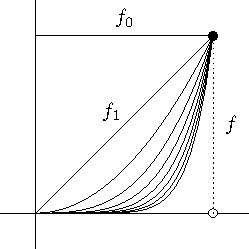
\includegraphics{images/discontinuous-limit}
        \caption{Die Funktionenfolge in Beispiel (3)}%
        \label{fig:discontinuous-limit}
      \end{figure}
    \item Betrachte die Funktionen $f_n \colon \mathbb{R} \to \mathbb{R}$ mit $f_n(x) = \sin(nx)$.
      Für $x = \pi/2$ gilt
      \[
        f_n(\pi/2) = \sin(n/2 \cdot \pi)
        =
        \begin{cases}
          0 & n = 0, 2, 4, 6, \dots,\\
          1 & n = 1, 5, 9, \dots,\\
          -1 & n = 3, 7, 11, \dots.
        \end{cases}
      \]
      Insbesondere existiert der Grenzwert
      \(
      \lim_{n \to \infty} f_n(\pi/2)
      \)
      nicht. Es existiert also keine Funktion
      $f \colon \mathbb{R} \to \mathbb{R}$ 
      mit
      \(
        \lim_{n \to \infty} f_n = f.
      \)
      In anderen Worten konvergiert die
      Funktionenfolge ${(f_{n})}_{n \in \mathbb{N}}$ nicht.
    \item Betrachte die Funktionen
      $f_n \colon \mathbb{R} \to \mathbb{R}$ 
      mit
      \[
        f_n(x) = \sum_{k=1}^{n} \frac{1}{k^2}\sin(kx).
      \]
      Wir erinnern uns, dass die Reihe
      $\sum_{k=0}^{\infty} 1/k^2$ konvergiert.
      Sei $\varepsilon > 0$. Dann existiert
      $N \in \mathbb{N}$ mit
      \[
        \sum_{k=N}^{\infty} \frac{1}{k^2} \leq \varepsilon.
      \]
      Für $n \geq m \geq N$ und alle $x \in \mathbb{R}$ 
      gilt dann
      \[
        |f_n(x) - f_m(x)| =
        \left| \sum_{k=m+1}^{n} \frac{1}{k^2} \sin(kx) \right|
        \leq
        \sum_{k=m+1}^{n} \frac{1}{k^2} \leq
        \sum_{k=N}^{\infty} \frac{1}{k^2} \leq \varepsilon.
      \]
      Also ist für alle
      $x \in \mathbb{R}$ 
      die Folge ${(f_{n}(x))}_{n \in \mathbb{N}}$
      eine Cauchyfolge in $\mathbb{R}$,
      also konvergent.
      Wir schliessen, dass die Funktionenfolge
      ${(f_{n})}_{n \in \mathbb{N}}$ auf $\mathbb{R}$ 
      konvergiert, mit Grenzfunktion
      $f \colon \mathbb{R} \to \mathbb{R}$.
      Wir werden bald sehen, dass $f$ stetig ist.
      Es ist jedoch schwierig, die Funktion
      $f$ konkreter zu beschreiben. Wir wissen jedoch,
      dass $f$ periodisch ist mit Periode $2\pi$,
      das heisst, für alle $x \in \mathbb{R}$ gilt
      $f(x + 2\pi) = f(x)$.
      Dazu bemerke bloss, dass für alle $n \in \mathbb{N}$ 
      gilt, dass $f_n(x + 2 \pi) = f_n(x)$.
  \end{enumerate}
\end{examples}

Wir untersuchen nun einen Konvergenzbegriff für Funktionenfolgen,
der sicher stellen soll, dass die Grenzfunktion einige gute Eigenschaften
der einzelnen Glieder erbt.

\begin{definition}
  Sei $X \subset \mathbb{R}$ eine beliebige Teilmenge.
  Eine Folge ${(f_{n})}_{n \in \mathbb{N}}$ von Funktionen $f_n \colon X \to \mathbb{R}$
  \emph{konvergiert gleichmässig} mit Grenzfunktion $f \colon X \to \mathbb{R}$,
  falls für alle $\varepsilon > 0$ ein Index $N \in \mathbb{N}$ existiert,
  so dass für alle $n \geq N$ und alle $x \in X$ gilt, dass
  $|f_n(x) - f(x)| \leq \varepsilon$.
\end{definition}

Dies unterscheidet sich von der üblichen (punktweisen) Konvergenz dadurch,
dass bei der gleichmässigen Konvergenz der Index $N$ nicht vom Punkt $x$ abhängen darf.
Siehe auch Abbildung~\ref{fig:uniform}.

\begin{figure}[htb]
  \centering
  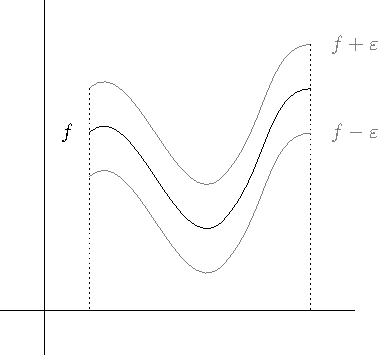
\includegraphics{images/uniform}
  \caption{Gleichmässige Konvergenz heisst, dass sich jedes
  $f_n$ im $\varepsilon$-breiten Band um $f$ befindet.}%
  \label{fig:uniform}
\end{figure}

\begin{examples}
  \leavevmode
  \begin{enumerate}[(1)]
    \item Sei $X = [0, 1]$ und betrachte die Funktionen
      \begin{align*}
        f_n \colon [0, 1] & \to \mathbb{R} \\
        x & \mapsto x^n.
      \end{align*}
      Die Folge ${(f_{n})}_{n \in \mathbb{N}}$ konvergiert
      punktweise gegen die Funktion
      \begin{align*}
        f \colon [0, 1] & \to \mathbb{R} \\
        x & \mapsto
        \begin{cases}
          0 & x < 1,\\
          1 & x = 1.
        \end{cases}
      \end{align*}
      Diese Konvergenz ist jedoch nicht gleichmässig.
      Sei dazu $\varepsilon = 1/3$.
      Bemerke, dass alle $f_n \colon [0, 1] \to \mathbb{R}$ stetig sind.
      Nach dem Zwischenwertsatz existiert also $x_n \in (0, 1)$ 
      mit $f_n(x_n) = 1/2$.
      Es folgt, dass
      \[
        |f_n(x_n) - f(x_n)| = |1/2 - 0| = 1/2.
      \]
      Wir schliessen, dass kein $N \in \mathbb{N}$ existiert, so dass
      für alle $x \in [0, 1]$ gilt, dass \[|f_n(x) - f(x)| \leq 1/3.\]
    \item Sei $a \in (0, 1)$.
      Betrachte die Funktionen
      \begin{align*}
        f_n \colon [0, a] & \to \mathbb{R} \\
        x & \mapsto x^n.
      \end{align*}
      Dann konvergiert die Funktionenfolge ${(f_{n})}_{n \in \mathbb{N}}$ 
      gleichmässig gegen die Nullfunktion $f \colon[0, a] \to \mathbb{R}$.
      Sei dazu $\varepsilon > 0$ vorgegeben. Wähle $N \in \mathbb{N}$ mit
      $a^N \leq \varepsilon$. Ein solches $N$ existiert, da $a < 1$.
      Dann gilt für alle $n \geq N$ und alle $x \in [0, a]$, dass
      \[
        |f_n(x) - f(x)| = |x^n - 0| = x^n \leq a^n \leq a^N \leq \varepsilon.
      \]
    \item Seien $a_0, a_1, a_2, \dots$  und $b_1, b_2, b_3, \dots$ reelle Zahlen,
      so dass
      \[
        \sum_{k=1}^{\infty} |a_k| + |b_k| < \infty.
      \]
      Definiere $f_n \colon \mathbb{R} \to \mathbb{R}$ durch
      \[
        f_n(x) = a_0 + \sum_{k=1}^{n} a_k \cos(kx) + b_k \sin(kx).
      \]
      Dann konvergiert die Funktionenfolge $f_n$ gleichmässig gegen die
      Grenzfunktion
      \[
        f(x) = a_0 + \sum_{k=0}^{\infty} a_k \cos(kx) + b_k \sin (kx).
      \]
      Sei dazu $\varepsilon > 0$.
      Wähle $N \in \mathbb{N}$ mit
      \[
        \sum_{k=N}^{\infty} |a_k| + |b_k| \leq \varepsilon.
      \]
      Dann gilt für alle $n \geq N$ und alle $x \in \mathbb{R}$, dass
      \[
        |f_n(x) - f(x)| = \left| \sum_{k = n + 1}^{\infty} a_k \cos(kx)
        + b_k \sin (kx)\right| \leq \sum_{k=N}^{\infty} |a_k| + |b_k| \leq \varepsilon.
      \]

      Ein explizites Beispiel dafür ist
      \[
        f_n(x) = \sum_{k=1}^{n} \frac{\cos(kx)}{k^2}.
      \]
      Für die Grenzfunktion $f \colon\mathbb{R} \to \mathbb{R}$ gilt dann
      \[
        f(x) = \frac{\pi^2}{6} - \frac{\pi}{2}x + \frac{x^2}{4}
      \]
      für $x \in [0, 2 \pi]$. Weiterhin ist die Funktion
      $f \colon \mathbb{R} \to \mathbb{R}$ periodisch mit Periode
      $2 \pi$, das heisst für alle $x \in \mathbb{R}$ gilt $f(x + 2\pi) = f(x)$.
      Siehe auch Abbildung~\ref{fig:pi-squared-sixths}.
      Wir werden das noch genauer untersuchen, sobald wir Fourierreihen studieren.
      
      \begin{figure}[htb]
        \centering
        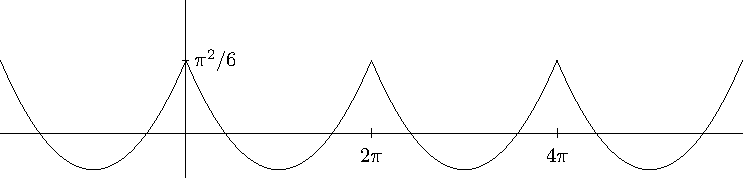
\includegraphics{images/pi-squared-sixths}
        \caption{Eine $2\pi$-periodische Funktion $f$
        mit $f(x) = \pi^2/6 - \pi/2 \cdot x + x^2/4$
      für alle $x \in [0, 2\pi]$.}%
        \label{fig:pi-squared-sixths}
      \end{figure}
  \end{enumerate}
\end{examples}

\begin{theorem}[Satz von Weierstrass]\label{thm:weierstrass}
  Sei ${(f_{n})}_{n \in \mathbb{N}}$ eine Folge von stetigen Funktionen
  $f_n \colon X \to \mathbb{R}$, welche gleichmässig gegen
  $f \colon X \to \mathbb{R}$ konvergiert.
  Dann ist $f$ stetig.
\end{theorem}

\begin{proof}
  Die Idee in diesem Beweis ist $\varepsilon$ zu dritteln.
  Sei $p \in X$ und $\varepsilon > 0$ vorgegeben.
  Wähle $N \in \mathbb{N}$ so, dass für alle $n \geq N$ 
  und $x \in X$ gilt, dass
  $|f_n(x) - f(x)| \leq \varepsilon /3$.
  Wähle $\delta > 0$ so, dass
  für alle $x \in X$ mit $|x - p| \leq \delta$ gilt,
  dass
  \(
    |f_N(x) - f_N(p)| \leq \varepsilon/3.
  \)
  Das geht, da $f_N$ stetig ist.
  Dann gilt für alle $x \in X$ mit $|x - p| \leq \delta$, dass
  \begin{align*}
    |f(x) - f(p)| &= |f(x) - f_N(x) + f_N(x) - f_N(p) + f_N(p) - f(p)| \\
                  & \leq |f(x)  -f_N(x)| + |f_N(x) - f_N(p)| + |f_N(p) - f(p)|\\
                  & \leq \varepsilon/3 + \varepsilon/3 + \varepsilon/3 = \varepsilon.
  \end{align*}
  Also ist $f$ stetig im Punkt $p \in X$.
\end{proof}

\begin{proposition}\label{prop:power-series-uniform}
  Sei 
  \(
    P(x) = \sum_{k=0}^{\infty} a_k x^k
  \)
  eine Potenzreihe mit Konvergenzradius $r > 0$.
  Sei weiterhin $s > 0$ mit $s < r$.
  Dann konvergiert die Funktionenfolge ${(f_{n})}_{n \in \mathbb{N}}$ mit
  \[
    f_n(x) = \sum_{k=0}^{n} a_k x^k
  \]
  auf dem Intervall $[-s, s]$ gleichmässig gegen die Funktion
  $f \colon [-s, s] \to \mathbb{R}$ mit
  \[
    f(x) = \sum_{k=0}^{\infty} a_k x^k.
  \]
  Insbesondere ist die Grenzfunktion $f \colon [-s, s] \to \mathbb{R}$ stetig.
\end{proposition}


\begin{proof}
  Aus dem Beweis von Theorem~\ref{thm:hadamard} wissen wir, dass die Reihe
  \(
    \sum_{k=0}^{\infty} a_k s^k
  \)
  absolut konvergiert, da $s < r$.
  Sei nun $\varepsilon > 0$ vorgegeben.
  Wähle $N \in \mathbb{N}$ so, dass
  \[
    \sum_{k=N}^{\infty} |a_k| s^k \leq \varepsilon.
  \]
  Für alle $n \geq N$ und alle $x \in [-s, s]$ gilt dann
   \begin{align*}
     |f_n(x) - f(x)|
     & = \left| \sum_{k=n+1}^{\infty} a_k x^k \right|\\
     & \leq \sum_{k=n+1}^{\infty} |a_k| \cdot |x|^k\\
     & \leq \sum_{k=N}^{\infty} |a_k| s^k \leq \varepsilon. 
  \end{align*}
  Also konvergiert die Funktionenfolge ${(f_{n})}_{n \in \mathbb{N}}$ auf $[-s, s]$ 
  gleichmässig gegen $f$.
\end{proof}

\begin{question}
  Was passiert im Grenzfall $x = \pm r$, wobei $r$ der Konvergenzradius ist?
\end{question}

Diese Frage ist interessant, da die Reihen $P(r)$ und $P(-r)$
im allgemeinen nicht konvergieren.

\begin{example}
  Betrachte
  \[
    P(x) = \sum_{k=0}^{\infty} x^k.
  \]
  Dann konvergieren $P(1)$ und $P(-1)$ nicht.
\end{example}


\begin{proposition}[Grenzwertsatz von Abel]\label{prop:abel-grenzwertsatz}
  Sei $r$ der Konvergenzradius der Potenzreihe
  \[
    P(x) = \sum_{n=0}^{\infty} a_n x^n.
  \]
  Falls $P(r)$ konvergiert, dann konvergiert die Folge
  ${(f_{n})}_{n \in \mathbb{N}}$ mit
  \(
    f_n(x) = \sum_{k=0}^{n}  a_k x^k
  \)
  auf $[0, r]$ gleichmässig gegen die Grenzfunktion $f \colon [0, r] \to \mathbb{R}$
  mit
  \(
    f(x) = \sum_{k=0}^{\infty} a_k x^k.
  \)
  Insbesondere ist $f \colon [0, r] \to \mathbb{R}$ stetig.
\end{proposition}

\begin{example}
  Die Formel
  \[
    \log(1 + x) = \sum_{k=0}^{\infty} {(-1)}^k \frac{x^{k+1}}{k+1}
  \]
  gilt für alle $x \in (-1, 1)$.
  Wir bemerken, dass
  \[
    P(1) = 1 - 1/2 + 1/3 - 1/4 + \cdots
  \]
  konvergiert (aber nicht absolut).
  Aus Proposition~\ref{prop:abel-grenzwertsatz} folgt
  \[
    \log(2) = \lim_{x \to 1} \log(1 + x)
    = \lim_{x \to 1} P(x) = P(1).
  \]
  Wir schliessen, dass
  \[
    \log(2) = 1 - 1/2 + 1/3 - 1/4 + \cdots.
  \]
\end{example}

\begin{proof}[Beweis von Proposition~\ref{prop:abel-grenzwertsatz}]
  Wir führen den Beweis im Spezialfall $r = 1$.
  Der allgemeine Fall kann durch eine Skalierung leicht auf diesen
  Fall reduziert werden.
  Berechne für alle $x \in [0, 1]$ und alle $n, k \in \mathbb{N}$, dass
  \begin{align*}
    f_{n+k}(x) - f_n(x) 
    &= a_{n+1}x^{n+1} + a_{n+2}x^{n+2} + \cdots + a_{n+k}x^{n+k} \\
    & = (a_{n+1} + a_{n+2} + \cdots + a_{n+k}) \cdot x^{n+k}\\
    &\;\;\;\;\; + (a_{n+1} + a_{n+2} + \cdots + a_{n+k-1}) \cdot (x^{n+k-1} - x^{n+k})\\
    &\;\;\;\;\; + (a_{n+1} + a_{n+2} + \cdots + a_{n+k - 2}) \cdot (x^{n+k-2} - x^{n+k-1})\\
    &\;\;\;\;\; + \cdots
    + a_{n+1} \cdot (x^{n+1} - x^{n+2}).
  \end{align*}
  Dieser ``Höllensumme'' sagt man \emph{Abel Summation}.
  Da die Reihe $\sum_{k=0}^{\infty} a_k$ konvergiert,
  existiert zu jedem $\varepsilon > 0$ ein $N \in \mathbb{N}$, so
  dass für alle $n \geq N$ und alle $k \in \mathbb{N}$ gilt, dass
  $|a_{n+1} + a_{n+2} + \cdots + a_{n+k}| \leq \varepsilon$.
  Für alle $x \in [0, 1]$, alle $n \geq N$ und alle $k \in \mathbb{N}$ gilt nun, dass
  \begin{align*}
    |f_{n+k}(x) - f_n(x)| 
    &\leq \varepsilon x^{n+k} +
    \varepsilon \cdot (x^{n+k-1} - x^{n+k}) + \cdots + \varepsilon \cdot (x^{n+1} - x^{n+2})\\
    &\leq \varepsilon x^{n+1}\\ & \leq \varepsilon.
  \end{align*}
  Im Grenzübergang $k \to \infty$ erhalten wir, dass $|f(x) - f_n(x)| \leq \varepsilon$
  für alle $x \in [0, 1]$ und alle $n \geq N$.
\end{proof}


% Bevor wir Proposition~\ref{prop:swap-limit-integral} beweisen, betrachten wir
% eine alternative Definition der gleichmässigen Konvergenz.

% \begin{definition}
%   Die Folge ${(f_{n})}_{n \in \mathbb{N}}$ von Funktionen $f_n \colon X \to \mathbb{R}$ 
%   heisst gleichmässig konvergent, falls für alle $\varepsilon > 0$ 
%   ein $N \in \mathbb{N}$ existiert, so dass für alle
%   $n, m \geq N$ und alle  $x \in X$ gilt, dass $|f_n(x) - f_m(x)| \leq \varepsilon$.
% \end{definition}

% Dass die beiden Definitionen äquivalent sind, liegt lediglich an der
% Vollständigkeit von $\mathbb{R}$.
% Der Vorteil dieser Definition gegenüber der ursprünglichen ist,
% dass die Grenzfunktion $f \colon X \to \mathbb{R}$ nicht im Voraus bekannt zu sein braucht.

% \begin{example}
%   Sei $P(x) = \sum_{k=0}^{\infty} a_k x^k$ mit $a_k \in \mathbb{R}$ mit Konvergenzradius $r > 0$.
%   Für $s \in (0, r)$ ist die Funktionenfolge ${(f_{n})}_{n \in \mathbb{N}}$ mit
%   $f_n(x) = \sum_{k=0}^{n} a_k x^k$ auf dem Intervall $[-s, s]$ 
%   gleichmässig konvergent, mit Grenzfunktion $f \colon [-s, s] \to \mathbb{R}$, wobei
%   $f(x) = \sum_{k=0}^{\infty} a_k x^k$.
%   Siehe dazu Theorem~\ref{thm:weierstrass} und Proposition~\ref{prop:power-series-uniform}.
% \end{example}

\subsection*{Gliedweise Integration}
\begin{question}
  Wann gilt
  \[
    \lim_{n \to \infty} \int_{a}^{b} f_n(x) \, dx = \int_{a}^{b} \lim_{n \to \infty} f(x)\, dx?
  \]
\end{question}

\begin{proposition}\label{prop:swap-limit-integral}
  Sei ${(f_{n})}_{n \in \mathbb{N}}$ eine Folge stetiger Funktionen
  $f_n \colon [a, b] \to \mathbb{R}$, welche gleichmässig
  gegen $f \colon[a, b] \to \mathbb{R}$ konvergiert. Dann gilt
  \[
    \lim_{n \to \infty} \int_{a}^{b} f_n(x) \, dx = \int_{a}^{b} f(x) \, dx.
  \]
\end{proposition}

\begin{proof}[Beweis von Proposition~\ref{prop:swap-limit-integral}]
  Wir bemerken zuerst, dass $f \colon [a, b] \to \mathbb{R}$ stetig, also auch
  Riemann-integrierbar ist.
  Sei $\varepsilon > 0$ vorgegeben.
  Wähle $N \in \mathbb{N}$ so, dass für alle $n \geq N$ und alle $x \in [a, b]$ gilt,
  dass
  $|f_n(x) - f(x)| \leq \varepsilon/(b-a)$.
  Dann gilt für $n \geq N$, dass
  \[
     \left| \int_{a}^{b} f_n(x) \, dx - \int_{a}^{b} f(x) \, dx\right|  
     = \left| \int_{a}^{b} f_n(x) - f(x) \, dx \right|  
     \leq \int_{a}^{b} |f_n(x) - f(x) \, dx \leq \varepsilon.\qedhere
  \]
\end{proof}

\begin{example}
  Sei $P(x) = \sum_{k=0}^{\infty} a_k x^k$ eine Potenzreihe mit Konvergenzradius $r > 0$.
  Sei $s \in (0, r)$ und $[a, b] \subset [-s, s]$. Dann gilt
  \begin{align*}
    \int_{a}^{b} \sum_{k=0}^{\infty}  a_k x^k \, dx 
    &= \lim_{n \to \infty} \int_{a}^{b} \sum_{k=0}^{n} a_k x^k \, dx  \\
    &=  \lim_{n \to \infty} \sum_{k=0}^{n} \int_{a}^{b} a_k x^k \, dx \\
    &= \sum_{k=0}^{\infty} a_k \cdot \frac{b^{k+1} - a^{k+1}}{k+1}.
  \end{align*}
  Für das Vertauschen des Limes mit dem Integral haben wir 
  Propositionen~\ref{prop:power-series-uniform} und~\ref{prop:swap-limit-integral} benutzt.
  Wir schliessen, dass gliedweise Integration innerhalb des Konvergenzbereichs
  von $P(x)$ erlaubt ist.
\end{example}

\subsection*{Gliedweise Ableitung}
\begin{question}
  Wann gilt
  \[
    \lim_{n \to \infty} f_n' = \left(\lim_{n \to \infty} f_n \right)'?
  \]
\end{question}

\begin{example}
  Betrachte die Funktionenfolge ${(f_{n})}_{n \in \mathbb{N}}$ mit
  $f_n(x) = 1/n \cdot \cos(nx)$.
  Dann konvergiert ${(f_{n})}_{n \in \mathbb{N}}$ gleichmässig auf $\mathbb{R}$ 
  gegen die Nullfuktion. Aber
  die Folge der Ableitungen $f_n'(x) = -\sin (nx)$ konvergiert nicht,
  insbesondere nicht gegen die Nullfunktion.
  Die Details dazu werden auf Serie~12 ausgearbeitet.
  In diesem Fall können wir den Limes also nicht mit der Ableitung vertauschen.
\end{example}

\begin{proposition}\label{prop:derivative-uniform}
  Seien $f_n \colon (a, b) \to~\mathbb{R}$ stetig differenzierbare
  Funktionen, so dass
  \begin{enumerate}[\normalfont(i)]
    \item die Folge $f_n' \colon (a, b) \to \mathbb{R}$ gleichmässig gegen
      eine Funktion $g \colon (a, b) \to \mathbb{R}$ konvergiert,
    \item für mindestens einen Punkt $p \in (a, b)$ der Grenzwert
      $\lim_{n \to \infty} f_n(p) \in \mathbb{R}$ existiert.
  \end{enumerate}
  Dann konvergiert die Folge  ${(f_{n})}_{n \in \mathbb{N}}$ gleichmässig
  gegen eine differenzierbare Funktion $f \colon (a, b) \to \mathbb{R}$,
  und es gilt $f' = g$.
\end{proposition}

\begin{proof}
  Wir zeigen die Proposition in zwei Schritten. Im ersten Schritt zeigen wir,
  dass ${(f_{n})}_{n \in \mathbb{N}}$ gleichmässig auf $(a, b)$ konvergiert.
  Dazu sei $\varepsilon > 0$ vorgegeben. Seien $m, n \in \mathbb{N}$ 
  mit $m > n$, und sei $x \in (a, b)$.
  Betrachte die Hilfsfunktion
  \(
    h(x) = f_m(x) - f_n(x)
  \).
  Nach dem Mittelwertsatz existiert $ t$ zwischen $p$ und $x$ mit
  $h(x) =  h(p) + h'(t) \cdot (x - p)$.
  Wähle $N_1 \in \mathbb{N}$ so, dass für alle $n , m \geq N_1$ und
  alle $t \in (a, b)$ gilt, dass
  \[
  |f_n'(t) - f_m'(t)| \leq \frac{\varepsilon }{2(b-a)}.
  \]
  Wähle $N_2 \in \mathbb{N}$ so, dass für alle $n , m \geq N_2$ gilt,
  dass
  \(
    |f_n(p) - f_m(p)| \leq \varepsilon/2
  \).
  Für alle $x \in (a, b)$ und alle $n, m \geq N = \max\{N_1, N_2\}$ gilt dann
   \begin{align*}
     h(x) 
     &\leq |h(p)| + |h'(t)| \cdot |x - p|  \\
     &= |f_m(p) - f_n(p)| + |f_m'(t) - f_n'(t)| \cdot |x - p| \\
     & \leq \frac{\varepsilon}{2} + \frac{\varepsilon}{2(b-a)}\cdot (b-a) = \varepsilon.
  \end{align*}
  Also gilt für alle $x \in (a, b)$ und alle $n, m \geq N$, dass
  $|f_m(x) - f_n(x)| \leq \varepsilon$. Da $\mathbb{R}$ vollständig ist,
  bedeutet das, dass ${(f_{n})}_{n \in \mathbb{N}}$ gleichmässig konvergent ist.
  Sei also $f$ die Grenzfunktion.
  
  Im zweiten Schritt zeigen wir nun, dass $f$ differenzierbar ist, und
  dass $f' = g$ gilt.
  Dazu machen mir einen Ansatz für eine Dreigliedentwicklung von $f$
  an der Stelle $x \in (a, b)$. Schreibe
  \[
    f(x + h) = f(x) + g(x) \cdot h + {(Rf)}_x(h).
  \]
  Zu zeigen ist, dass ${(Rf)}_x(h)$ relativ klein in $|h|$ ist.
  Sei dazu $n \in \mathbb{N}$.
  Nach dem Mittelwertsatz existiert $t$ zwischen $x$ und $x + h$ 
  so, dass $f_n(x + h) = f_n(x) + f_n'(t) \cdot h$.
  Umgeschrieben heisst das, dass
  \[
    f_n(x + h) = f_n(x) + f_n'(x) \cdot h + (f_n'(t) - f_n'(x)) \cdot h.
  \]
  Schreibe ${(Rf_n)}_x(h) = (f_n'(t) - f_n'(x)) \cdot h$.
  Wähle $N \in \mathbb{N}$ so, dass für alle $n, m \geq N$ und alle
  $t \in (a, b)$ gilt, dass $|f_m'(t) - f_n'(t)| \leq \varepsilon/3$.
  Weiter wähle $\delta > 0$ so, dass für alle $t \in (a, b)$ mit
  $|t - x| \leq \delta$ gilt, dass
  $|f_N'(t) - f_N'(x) \leq \varepsilon/3$ gilt. Das geht, da $f_N'$ stetig ist.
  Für $n \geq N$ gilt dann
  $|{(Rf_n)}_x(h)| = |f_n'(t) - f_n'(x)| \cdot |h|$.
  Berechne
  \begin{align*}
    |f_n'(t) - f_n'(x)|
    & \leq |f_n'(t) - f_N'(t)| + |f_N'(t) - f_N'(x)| + |f_N'(x) - f_n'(x)|\\
    &\leq \varepsilon/3 + \varepsilon/3 + \varepsilon/3 = \varepsilon.
  \end{align*}
  Also haben wir
  \(
    |{(Rf_n)}_{x}(h)| \leq \varepsilon \cdot |h|
  \).
  Für alle $n \geq N$ und alle $|h| \leq \delta$ erhalten wir nun, dass
  \[
    f_n(x + h) = f_n(x) + f_n'(x) \cdot h + {(Rf_n)}_x(h)
  \]
  mit $|Rf_n(x, h)| \leq \varepsilon \cdot |h|$.
  Entscheidend ist, dass das $\delta$ nicht von $n$ abhängt (sonst wäre das
  bloss die Definition der Differenzierbarkeit von $f_n$).
  Im Grenzwert gilt dann
  \[
    f(x + h) = f(x) + g(x) \cdot h + {(Rf)}_x(h)
  \]
  mit $|{(Rf)}_x(h) \leq \varepsilon \cdot |h|$.
\end{proof}

\begin{application}
  Sei $P(x) = \sum_{k=0}^{\infty} a_k x^k$ mit Konvergenzradius $r > 0$.
  Der Konvergenzradius von der formal abgeleiteten Potenzreihe
  \[
    P'(x) = \sum_{k=1}^{\infty} k a_k x^{k-1}
  \]
  ist auch $r$, siehe Serie 12.
  Der springende Punkt hier ist, dass
  \[
    \lim_{n \to \infty} \sqrt[n]{n} = 1
  \]
  gilt. Für $s \in (0, r)$ konvergieren sowohl $P(x)$ als auch
  $P'(x)$ auf dem Intervall $[-s, s]$ gleichmässig gegen stetige Funktionen
  $f$ und $g$.
  Nach Proposition~\ref{prop:derivative-uniform} ist $f$ differenzierbar
  und $f' = g$.
  Wir schliessen, dass gliedweise Ableitung innerhalb des Konvergenzbereichs von
  $P(x)$ erlaubt ist.
\end{application}

\begin{example}
  Sei $f \colon \mathbb{R} \to \mathbb{R}$ unendlich oft differenzierbar und
  $Tf(x)$ die Taylorreihe von $f(x)$ mit Konvergenzradius $r \in [0, \infty]$.
  Dann definiert $Tf(x)$ auf $(-r, r)$ eine unendlich oft differenzierbare Funktion
  Das Problem hier ist, dass $Tf(x) $ und $f(x)$ auf $(-r, r)$ im allgemeinen
  nicht übereinstimmen:
  Zum Beispiel ist die Taylorreihe von
  \[
    f(x) =
    \begin{cases}
      e^{-1/x^2} & x \neq 0\\
      0 & x = 0
    \end{cases}
  \]
  identisch null, also ist $f(x)$ nicht durch $Tf(x)$ bestimmt.
\end{example}
\end{document}
